% !TEX encoding = UTF-8 Unicode
%!TEX TS-program = xelatex

\documentclass[12pt]{extarticle}
% extarticle is like article but can handle 8pt, 9pt, 10pt, 11pt, 12pt, 14pt, 17pt, and 20pt text

\def \ititle {Origins of Mind}
 
\def \isubtitle {Lecture 08}
 
\def \iauthor {Stephen A. Butterfill}
\def \iemail{s.butterfill@warwick.ac.uk}
\date{}

%for strikethrough
\usepackage[normalem]{ulem}

\usepackage{pdfpages}


\input{$HOME/Documents/submissions/preamble_steve_handout}

%logic symbol \leftmodels
\usepackage{MnSymbol}

%\bibpunct{}{}{,}{s}{}{,}  %use superscript TICS style bib
%remove hanging indent for TICS style bib
%TODO doesnt work
\setlength{\bibhang}{0em}
%\setlength{\bibsep}{0.5em}


%itemize bullet should be dash
\renewcommand{\labelitemi}{$-$}

\begin{document}

%\raggedcolumns

\begin{multicols*}{3}

\setlength\footnotesep{1em}


\bibliographystyle{newapa} %apalike

%\maketitle
%\tableofcontents




%--------------- 
%--- start paste
\def \ititle {Logic I}
 
\def \isubtitle {Lecture 18}
 
\begin{center}
 
{\Large
 
\textbf{\ititle}: \isubtitle
 
}
 
 
 
\iemail %
 
\end{center}
 
Readings refer to sections of the course textbook, \emph{Language, Proof and Logic}.
 
 
 
\section{Proofs about Proofs}
 
\begin{minipage}{\columnwidth}
 
\textbf{If A $\vdash$ B then $\vdash$ A→B}
 
Proof Given a proof for A $\vdash$ B …
 
\begin{center}
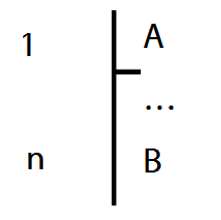
\includegraphics[scale=0.3]{img/unit_440_a.png}
\end{center}
… we can turn it into a proof for $\vdash$ A→B:
 
\begin{center}
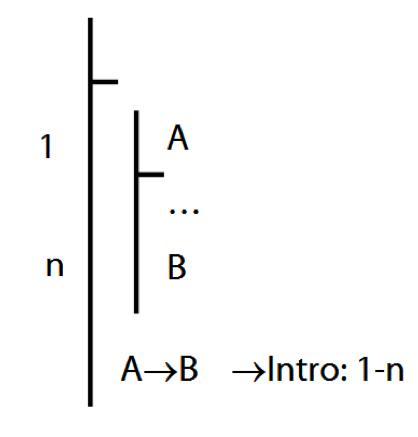
\includegraphics[scale=0.3]{img/unit_440_b.png}
\end{center}
\end{minipage}
 
\textbf{If $\vdash$ A→B then A $\vdash$ B}
 
\begin{minipage}{\columnwidth}
 
\textbf{If A $\vdash$ B then A $\vdash$ ¬¬B}
 
Proof:
 
\begin{center}
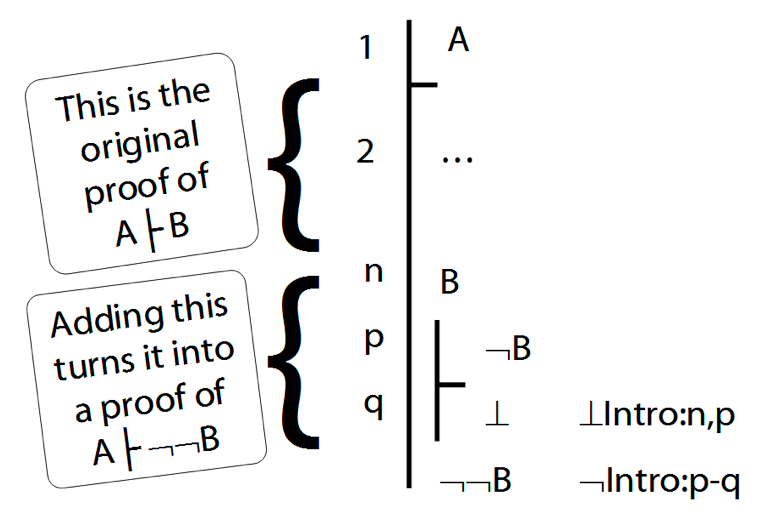
\includegraphics[scale=0.3]{img/unit_440_c.png}
\end{center}
\end{minipage}
 
\textbf{If A $\vdash$ C then A $\vdash$ B→C}
 
\textbf{If A $\vdash$ B and A $\vdash$ ¬C then A $\vdash$ ¬(B→C)}
 
 
 
\section{A $\vDash$ $\bot$}
 
 
 
\section{If (A $\nvdash$ $\bot$ entails A $\nvDash _{TT}$ $\bot$) then (A $\vDash_{TT}$ B entails A $\vdash$ B) }
 
First we show that if \textbf{A}, ¬B $\vdash$ $\bot$ then \textbf{A} $\vdash$ B .
 
(To do this, we show how to turn transform a proof of the former kind into a proof of the latter kind.)
 
Now assume that for all sets \textbf{A}, \textbf{A} $\nvdash$ $\bot$ entails \textbf{A} $\nvDash$$_{TT}$ $\bot$
 
Suppose that \textbf{A} $\vDash_{TT}$ B
 
Then \textbf{A}, ¬B $\vDash_{TT}$ $\bot$
 
So, by our assumption, \textbf{A}, ¬B $\vdash$ $\bot$
 
Therefore (by the thing we showed first) \textbf{A} $\vdash$ B
 
 
 
\section{The Essence of the Completeness Theorem}
 
\emph{Reading:} §8.3
 
\begin{center}
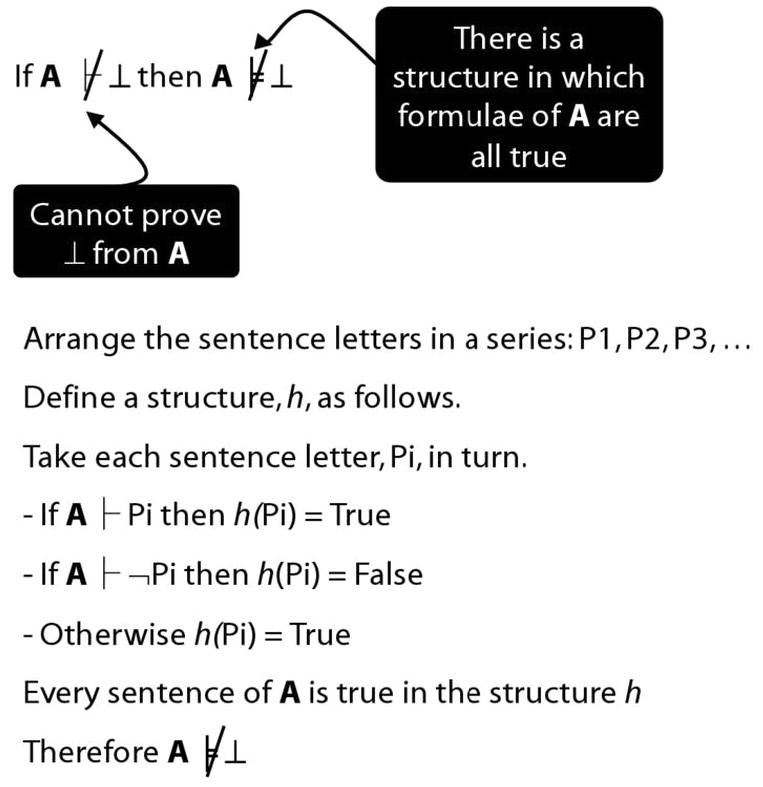
\includegraphics[scale=0.3]{img/unit_450.png}
\end{center}
 
 
\section{Lemma for the Completeness Theorem}
 
\emph{Reading:} §8.3
 
 
If for every sentence letter, P, either A $\vdash$ P or A $\vdash$ ¬P, then for every formula, X, either A $\vdash$ X or A $\vdash$ ¬X.
 
Proof
 
\textbf{Step a.} Suppose (for a contradiction) that there are formulae, X, such that A $\nvdash$ X and A $\nvdash$ ¬X. Take a shortest such formula, call it Y.
 
\textbf{Step b.} This formula, Y, must have one of the following forms: ¬P, P∨Q, P∧Q, P→Q, P↔Q, $\bot$
 
\textbf{Step c.} We can show that whichever form X has, either A $\vdash$ Y and A $\vdash$ ¬Y.
 
Case 1: X is P→Q. Then since P and Q are shorter than X, either:
 
\hspace{5mm} (i) A $\vdash$ P and A $\vdash$ ¬Q
 
\hspace{5mm} or
 
\hspace{5mm} (ii) A $\vdash$ ¬P
 
\hspace{5mm} or
 
\hspace{5mm} (iii) A $\vdash$ Q
 
\hspace{5mm} If (i), A $\vdash$ ¬(P→Q), that is, A $\vdash$ ¬X.
 
\hspace{5mm} If (ii), A $\vdash$ P→Q, that is, A $\vdash$ ¬X.
 
\hspace{5mm} If (iii), A $\vdash$ P→Q, that is, A $\vdash$ ¬X.
 
\hspace{5mm} (Here we use the last two Proofs about Proofs, see earlier)
 
Case 2: X is ¬P.
 
\hspace{5mm} Then since P is shorter, A $\vdash$ P or A $\vdash$ ¬P.
 
\hspace{5mm} If A $\vdash$ P then A $\vdash$ ¬¬P so A $\vdash$ ¬X which would contradict our assumption. This is shown in the proofs about proofs above.
 
\hspace{5mm} If A $\vdash$ ¬P then A $\vdash$ X (because X is ¬P), which would contradict our assumption.
 
Case 3: …
 
\textbf{Step d.} The demonstration in Step c contradicts our assumption, so we can conclude that it is false. That is, either A $\vdash$ X and A $\vdash$ ¬X for every formula X.
 
 
 
\section{Proof of the Completeness Theorem}
 
\emph{Reading:} §8.3, §17.1, §17.2
 
\begin{center}
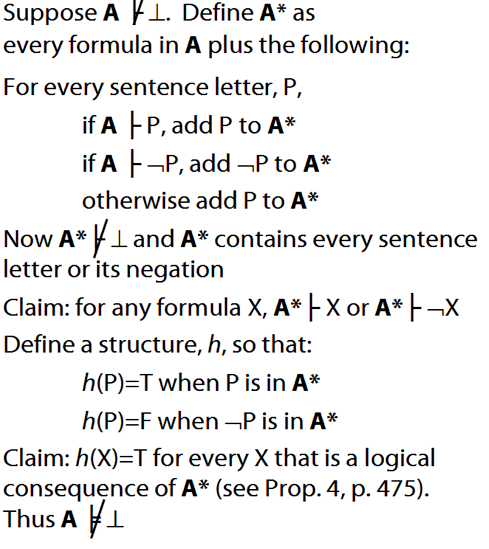
\includegraphics[scale=0.3]{img/unit_455_completeness.png}
\end{center}
 
 
\section{Proof of Proposition 4 for the Completeness Theorem}
 
\emph{Reading:} §15.1, §15.6
 
\vfill
\begin{minipage}{\columnwidth}
\section{Exercises}
These exercises will be discussed in seminars the week after this lecture.
The numbers below refer to the numbered exercises in the course textbook, e.g.\ `1.1' refers to exercise 1.1. on page 39 of the second edition of \emph{Language, Proof and Logic}. Exercises marked `*' are optional.
 
\begin{quote}
15.33--15.40 (second edition)
 
\end{quote}
\end{minipage}
%--- end paste
%--------------- 
 


\end{multicols*}

\end{document}